
\chapter{Test theories and statistical models}
\label{ch:2}
**here** to modify
\par A test is a tool to measure students abilities. As with any other measurement instrument, its user wants the measurement to be comparable to other measurements. \\
This observation, which was made for the first time probably thousands of years ago, led to the development of standardised tests. A test is considered to be standardised when the test procedures are fixed in such a way that differences among testing conditions, times, and places, do not influence the scores. Every testee will be given "the same test". As this statement does not necessarily imply that every test taker faces the same set of questions, accuracy of the measurement, or test reliability, is an important issue. Also, in order to establish fairness of testing and decision making based upon the scores, it is reasonable to require that the test actually measures the concept as intended, that it is \textbf{valid}. \\
In order to fulfill the validity and reliability conditions, test development requires a systematic approach, in which assembly procedures play an important role. As argued by Downing (2006), several phases in such an approach can be distinguished:
project plan, content definition, test specifications, items development, item banking, pretesting, item bank calibration, test assembly, test production, test administration and reporting results. \\
Also the developments of computers enhabled national test agencies such as INVALSI to introduce computers in educational testing in 2018 and to apply new testing procedures such as the substitution of paper and pencil (P\&P) testing with computer base testing (CBT).
Several methods are used nowadays. A common practice is selection by hand, usually after item analysis either based upon classical test theory (CTT) or item response theory (IRT). Larger testing programs, however, have better access to resources like sophisticated item banking systems, opening the possibility to improve their test assembly process by means of automated test assembly. \\

\par Automated test assembly (ATA) has great advantages over manual test assembly. First, knowing that automated methods will be employed forces a rigorous definition of test specifications early on, reducing the need to repeat some phases of the test development process. But also, more importantly, the number of possible combinations of items is too large to guarantee optimal or near-optimal solutions by hand. Thus, operational costs are reduced while improving quality control. Especially item response theory provides a good framework for automated test assembly methods. On the other hand, concepts from classical test theory have proven to be more accessible for everyone involved without an expert background. The framework of CTT, however, is less flexible than the IRT framework. \\
until **here** 
\par This technical report discusses the methods implemented in INVALSI test assembly operations for building the national standardized tests administered in the 2017/2018 school year to grade 8 and grade 10 students with the aim to assess their ability in mathematics and reading subjects.\\
First, in this chapter several key theoretical issues are briefly introduced such as the classical test theory and item response theory.
The optimization models used in automated test assembly will be argued in the second chapter while in the last chapter we are going to show the specific features of the models applied by INVALSI in 2017/2018 school year for the national standardized tests for grade 8 and 10 in mathematics and reading together with the features of the software used to solve the models. 
\section{Test theories}\label{sec:test-theories}
\subsection{Classical test theory}
%**skip?**
\par Classical test theory was born only after the following three achievements or ideas were conceptualized: one, a recognition of the presence of errors in measurements, two, a conception of that error as a random variable, and third, a conception of correlation and how to index it. In 1904, Charles Spearman was responsible for figuring out how to correct a correlation coefficient for attenuation due to measurement error and how to obtain the index of reliability needed in making the correction.\cite{Traub97} Spearman's finding is thought to be the beginning of Classical Test Theory by some.\\
%**skip?** 
\par Classical test theory assumes that each person $n$ has a true score, $\tau_n$, that would be obtained it there were no errors in measurement. A person's true score is defined as the expected number-correct score over an infinite number of independent administrations of the test. Unfortunately, test users never observe a person's true score, only an observed score, $X_n$. It is assumed that observed score is equal to the true score plus some error $E_n$:
\begin{equation}
X_n = \tau_n+E_n
\end{equation}
Furthermore, because of their very nature, the measurement errors over repeated administrations are uncorrelated, as well as true scores and measurement errors, while the expected error is zero. 
\par Classical test theory is concerned with the relations between these three variables in the population. These relations are used to say something about the quality of test scores. In this regard, the most important concept is that of \emph{reliability}. 
The reliability of the observed test scores, denoted by $\rho^2_{X\tau}$, is defined as the squared correlation between true scores and observed scores. A lower bound for reliability under rather mild assumptions and hence a popular approximation to
this unobservable quantity is the Cronbach's $\alpha$. It is a coefficient for the internal consistency of a test; that is, the degree to which all item scores in a test correlate positively with one another. Cronbach's $\alpha$ can be written as
\begin{equation}
\alpha= \frac{k}{1-k}\left(1- \frac{\sum_{i=1}^{k}\sigma^2_i}{\sigma_X} \right)
\end{equation}
where $k$ is the test length, $\sigma^2_X$ the test variance and $\sigma_i$ the item variance computed as the variance of the scores obtained at the item $i$. Unfortunately this function is non-linear with respect to the items and hence is not actively used in the test assembly models, anyway it can be employed to assess the consistency of the assembly results.
Two other item properties play an important role in CTT: item difficulty and item discrimination.
For dichotomously scores items, the difficulty is defined as the expected score given by a randomly selected examinee from the population of interest and is denoted by $\text{ES}_i$ (usually it's called $\pi_i$ or p-value $p_i$). Item discrimination is operationalised as the point biserial correlation between item score and test score, for item $i$ nd test $t$ is denoted as $\rho_{it}$.\\
\par
As stated in \cite{Hamb91} classical test theory show various drawbacks, one of the most important or well-known shortcomings of classical test theory is that examinee characteristics and test characteristics cannot be separated: each can only be interpreted in the context of the other. Another shortcoming lies in the definition of reliability, the problem with this is that there are differing opinions of what parallel tests are and so various reliability coefficients provide either lower bound estimates of reliability or reliability estimates with unknown biases. A third shortcoming involves the standard error of measurement. The problem here is that, according to classical test theory, the standard error of measurement is assumed to be the same for all examinees. However, as Hambleton explains in his book, scores on any test are unequally precise measures for examinees of different ability, thus making the assumption of equal errors of measurement for all examinees implausible. A fourth, and final shortcoming of the classical test theory is that it is test oriented, rather than item oriented. In other words, classical test theory cannot help us make predictions of how well an individual or even a group of examinees might do on a test item.\\
\subsection{Item response theory}
\par{An exhausitve essay about item response theory (IRT) models can be found in \cite{HumbSwa85}. In this section we are going to discuss IRT models with the only intention to supply their fundamental ideas and mathematical notation needed to comprehend the coming sections. \\
A unidimensional IRT model for dichotomous items (e.g. correct-incorrect) expresses the probability of endorsing an item as a function of the underlying ability and a set of item parameters representing the item properties through a \textit{S}-shaped curve called item characteristic curve (ICC). This function is non linear in the ability and it is monotone increasing because the idea behind these models is that the higher a person is located on the latent trait the higher is the probability she/he will give a correct answer. Different IRT models are characterized by the item response type, the number of item parameters, the latent ability structure, and the functional form.
%Very briefly, an IRT model assumes that the performance of an examinee can be predicted or explained by latent (non observable) factors called "abilities". The influence on the abilities of respondents test scores and test items features is explicitly modeled by different sets of parameters, in particular the relationship between a person's responses and the latent factor underlying this response can be described by an item characteristic curve (ICC).\\
%An ICC gives the probability of a correct answer as a function of the latent ability by non linear functions, this function is motone increasing because the idea behind these models is that the higher a person is located on the latent trait the higher is the probability they will give a correct answer.}\\
%\par{We will focus on models for dichotomous items, i.e. responses have only two possible values: 0 or 1, correct or incorrect, in particular we will show the main features of the Rasch model that is the model applied by INVALSI for the National standardized test in the school year 2017/2018\footnote{Motivations for using this approach can be found in **here**}.\\
We focus here on the Rasch model \cite{Rasch19601980} which is used by INVALSI for the national standardized tests. The Rasch model, also known as the one-parameter logistic (1PL) model, has an ICC expressed by the following formula
%The above cited Rasch model (also called 1-parameter logistic or 1PL) has an ICC expressed by the following formula:

\begin{equation}
P_i(\theta)=\frac{\exp(\theta-b_i)}{1+ \exp(\theta-b_i)}
\end{equation}
where $P_i(\theta)$ is the probability of a correct answer to item $i$ for an examinee of ability level $\theta \in (-\infty,\infty)$, and the parameter $b_i \in (-\infty,\infty) $ represents the difficulty of the item $i$. An example of ICCs for the Rasch model is shown in Figure \ref{fig:icc}. Note that the curves differ only by their location on the ability scale: the easiest item is C1 while the most difficult one is the C4. In fact, the Rasch model assumes that the difficulty parameter is the only item characteristic that influences the examinee's performance.

%\begin{center}
\begin{figure}[h]
	\centering
	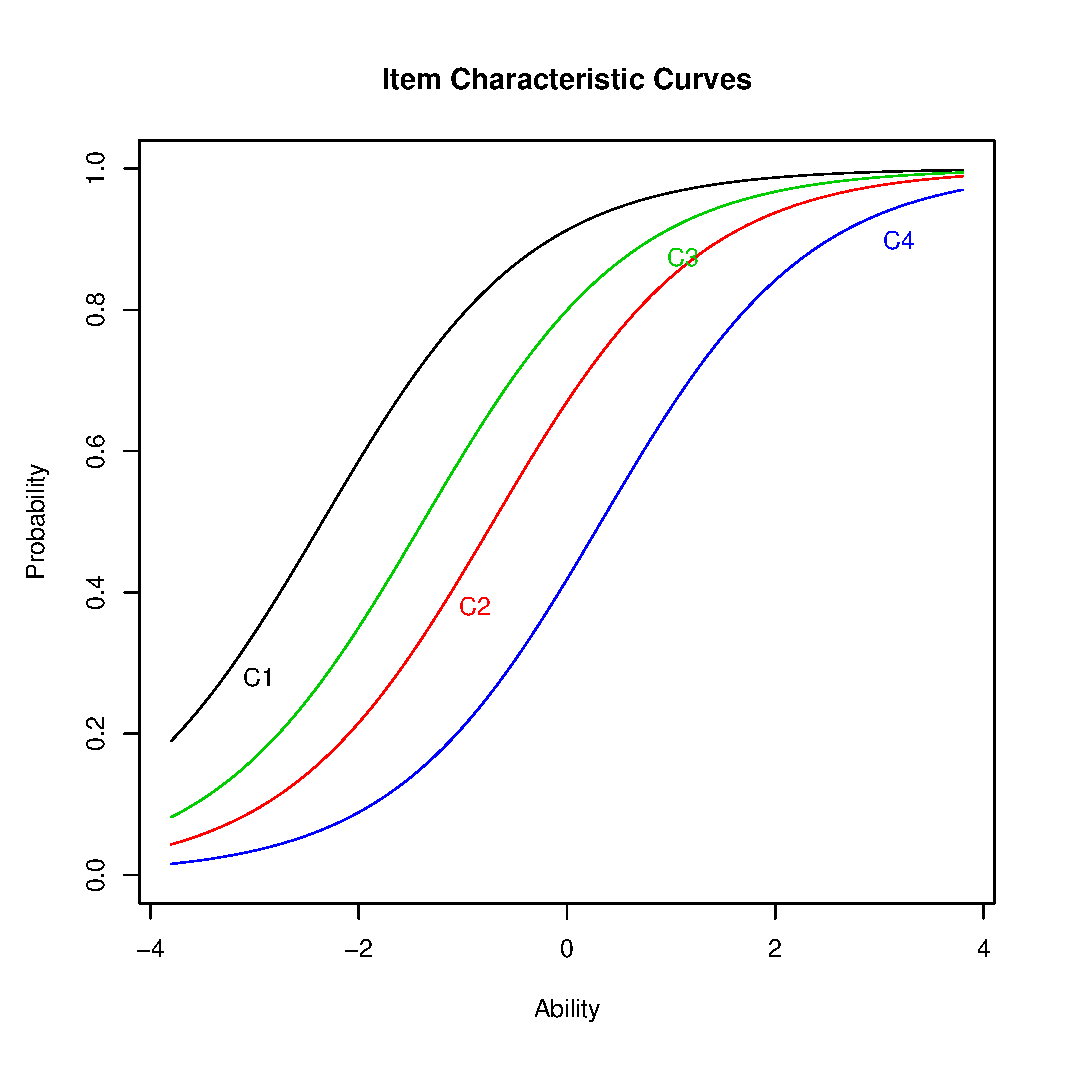
\includegraphics[scale=0.5]{Figures/icc.eps}
	\caption{ICCs of 4 items C1-C4 with different difficulties according to the Rasch model.}
	\label{fig:icc}
\end{figure}
%\end{center}

%to item $i$ for an examinee of ability level $\theta \in (-\infty,\infty)$
Some example of ICCs for the 1-parameter model are shown in Figure \ref{fig:ICCRasch}. The item parameters are as follows: for Item 1, $b_1 = 1.0$; for Item 2 $b_2 = 2.0$; for Item 3, $b_3 = -1.0$; and for Item 4, $b_4= 0.0$. Note that the curves differ only by their location on the ability scale. In the one-parameter model it is assumed that the item difficulty is the only item characteristic that influences examinee performance.\\
IRT models allow the simultaneous estimation of the item parameters and the examinees' abilities. The \textit{calibration} process usually involves the estimation of item parameters from pre-test response data. The \textit{scoring} phase deals with the estimation of the ability scores of the candidates. Once the item parameters have been estimated, it is possible to understand how precise the test is at various ranges of the latent ability by using the test information function (TIF), which is defined as the sum of the Fisher information for all the items in the test. In fact, under the maximum likelihood (ML) scoring, the Fisher information is asymptotically equal to the inverse of the variance of the ML estimator as follows
\subsubsection{Calibration}
\par{To use IRT models both the item parameters (difficulty $b$%**here%
	) and the examinees' abilities must be estimated, this process is usually called \emph{calibration} and it is performed in a separate phase before the main test, the so called \emph{pre-test}.	We refer to \cite{**here**} for any detail about calibration and hence pre-test estimation approaches applied by INVALSI in the school year 2017/2018.} \\
%\subsection{The Item bank}
%Before entering in the test assembly framework we should fix some notation and describe how the items are usually stored in a "database" called \emph{item bank} or \emph{item pool}
\par{Once the calibration has been done the items and their estimated and structural properties are stored in the \emph{item bank} (or pool) then we can move on to the test assembly procedure in which the items will be selected depending on those distinctive characteristics.\\
The Table \ref{fig:tabitembank} in the Tables chapter shows an example of the structure of an item bank of $I$ items, the items are displayed by row and in the columns we find the items features, from left to right: the identifier (\textsl{ID}), the IRT difficulty ($b$) together with its standard error ($b_{se}$), CTT expected score (\textsl{ES}), content attributes (\textsl{FORMAT}, \textsl{PROCESS}, \textsl{DOMAIN}) and relational attributes that specifies if the item belongs or not to a specific set (\textsl{ITEM SET 1}, \textsl{ITEM SET 2}, \textsl{ENEMY SET 1}, \textsl{ENEMY SET 2}, \textsl{ENEMY SET 3}).}\\
Examinees can get different sets of items because, thanks to the calibration and IRT models they can be placed on the scale created in the calibration phase and their scores can be still compared.\\
\subsubsection{Item and Test information functions}

In educational testing the precision of the ability estimator is tipically estimated using the variance of the estimates, in particular lower is the variance higher is the precision. Unfortunately the variance of the ability estimates in a nonlinear function of the items, therefore is more convenient in test assembly to use the Fisher information measure that asimptotically is the inverse of the variance of the estimator and moreover has a very favorable property that is the additivity (and hence linearity) over the items of a test. \\
\begin{equation}
I(\hat{\theta})=\frac{1}{\mathbb{V}(\hat{\theta})}
\end{equation}
In other words measuring the ability of the candidates as precisely as possible also comes down to maximising the Fisher information in the test (TIF) that is equal to the sum of the item information function (IIF) computed for each item in the test. For a test with $n$ items the TIF is equal to:
\begin{equation}
I(\theta)=\sum_{i=1}^n{I_i(\theta)}
\end{equation}
Finally expressions for the IIFs can be easily derived within the framework of IRT. For the 1PL model (Rasch) the item information function of the item $i$ is equal to:
\begin{equation}
I_i(\theta)=\frac{e^{\theta-b_i}}{(1+e^{\theta-b_i})^2}
\end{equation}
As we have already said tests can be assembled merely through selection of appropriate items out of an item bank, one way to do so is to use mathematical programming techniques (see for example \cite{Timminga 1989 and Adema 1990}) like 0-1 linear programming (LP) or mixed integer programming (MIP) models.\\
Using these approaches the tests can be built by, for instance, maximizing the TIF at predefined $\theta$ points (MAXIMIN in this report), or matching it with known optimal values (MINIMAX) with linear restrictions on the values of items properties.\\


 
 


